\documentclass[a4paper,12pt,twoside,titlepage]{article}

%Additional packages
\usepackage[utf8]{inputenc}
\usepackage[T1]{fontenc}
\usepackage[dutch,english]{babel}
\usepackage{syntonly}
\usepackage[official]{eurosym}
\usepackage{csquotes}

% Handle images
\usepackage{graphicx}
\graphicspath{ {./images/}{./styles/} }
\usepackage{float}
\usepackage{wrapfig}

% Handle URLs
\usepackage{xurl}
\usepackage{hyperref}
\hypersetup{colorlinks=true, linkcolor=blue, citecolor=blue, filecolor=blue, urlcolor=blue, pdftitle=, pdfauthor=, pdfsubject=, pdfkeywords=}

% Tables and listings
\usepackage{multirow,tabularx}
\usepackage[table]{xcolor} % Table colors
\usepackage{scrextend}
\addtokomafont{labelinglabel}{\sffamily}
\usepackage{listings}
\usepackage{adjustbox}

% Turn on indexing
\usepackage{imakeidx}
\makeindex[intoc]

% Define colors
\usepackage{color}
\definecolor{ashgrey}{rgb}{0.7, 0.75, 0.71}




% Listing style
\lstset{
  backgroundcolor=\color{ashgrey}, % choose the background color; you must add \usepackage{color} or \usepackage{xcolor}; should come as last argument
  rulecolor=\color{black},         % if not set, the frame-color may be changed on line-breaks within not-black text (e.g. comments (green here))
  frame=single,	                   % adds a frame around the code
  basicstyle=\footnotesize\ttfamily,  	   % the size of the fonts that are used for the code
  extendedchars=true,    	   % lets you use non-ASCII characters; for 8-bits encodings only, does not work with UTF-8
  breakatwhitespace=true, 	   % sets if automatic breaks should only happen at whitespace
  breaklines=true,        	   % sets automatic line breaking
  keepspaces=true,        	   % keeps spaces in text, useful for keeping indentation of code (possibly needs columns=flexible)
  columns=fullflexible,	  	   % Make sure no extra spaces are added.
  showstringspaces=false, 	   % if true show spaces in strings adding particular underscores
  showspaces=false        	   % show spaces everywhere adding particular underscores; it overrides 'showstringspaces'
}



\lstdefinestyle{DOS}
{
    backgroundcolor=\color{black},
    basicstyle=\scriptsize\color{white}\ttfamily
}

% Uncomment for production
% \syntaxonly

% Style
\pagestyle{headings}

% Define document
\author{D. Leeuw}
\title{Windows: Het systeem}
\date{\today\\
0.0.0
\vfill
\raggedright
\copyright\ 2025 Dennis Leeuw\\

%\begin{figure}

\includegraphics[width=0.3\textwidth]{CC-BY-SA-NC.png}
%\end{figure}

Dit werk is uitgegeven onder de Creative Commons BY-NC-SA Licentie en laat anderen toe het werk te kopi\"eren, distribueren, vertonen, op te voeren, en om afgeleid materiaal te maken, zolang de auteurs en uitgever worden vermeld als maker van het werk, het werk niet commercieel gebruikt wordt en afgeleide werken onder identieke voorwaarden worden verspreid.


}


\begin{document}
\selectlanguage{dutch}

\maketitle

%%%%%%%%%%%%%%%%%%%
%%% Introductie %%%
%%%%%%%%%%%%%%%%%%%

%%%%%%%%%%%%%%%%%
%%% De inhoud %%%
%%%%%%%%%%%%%%%%%

% requires: 
% provides: 
\section{Windows ontdekken}
Of je nu programmeur, helpdesk medewerker, systeembeheerder, hacker of security officer bent het is handig om te weten hoe een systeem werkt. Als programmeur is het essentieel om te weten welke functies een systeem je aanbiedt zodat je er gebruik van kan maken. Als hacker is het goed om te weten wat het systeem je biedt en wat de vaak voorkomende fouten zijn die programmeurs maken. Voor helpdesk medewerkers is het handig als je meer weet van de werking van een systeem zodat je makkelijker de fouten van gebruikers snapt en voor systeembeheerders is de kennis van de interne werking van een operating systeem nodig zodat het systeem en de bijbehorende software op een juiste en veilige manier ge\"installeerd kan worden. Ten slotte is het voor de security officer essentieel om al deze voorkomende zaken te begrijpen, zodat een juiste security analyse gemaakt kan worden.

We beschrijven in dit stuk de globale werking van het Windows besturingssysteem.


Besturingssytemen en software in zijn algemeen, wordt vaak beschreven in lagen, in het Engels layers\index{layer}. Een stapel van deze layers wordt in het Engels dan een stack\index{stack}.

De meest simpele vorm van een besturingssysteem stack is:
\begin{enumerate}
\item user applications\index{user applications}
\item operating system\index{operating system}
\item hardware\index{hardware}
\end{enumerate}

\begin{description}
\item[hardware] zijn de fysieke, tastbare, onderdelen van een computer. Hierbij horen CPU, geheugen, opslagsystemen, etc.
\item[operating system] ook bekent als OS\index{OS}, is een verzameling software die de hardware aanstuurt in opdracht van programma's (applications).
\item[user applications] ook bekent als apps\index{apps}, zijn de stukken software die wij, de gebruikers, gebruiken, zoals Microsoft Office.
\end{description}

De reden van het opdelen in lagen heeft meerdere redenen. Allereerst maakt het een complex geheel dat een operating system is overzichtelijk en makkelijker te begrijpen. Een andere reden is om te laten zien wat er afhankelijk is van elkaar. Bij operating systems heeft het ook te maken met een stukje veiligheid. Het operating system kan en mag tegen de hardware praten, terwijl user applications dat nu juist niet mogen. Het operating system bepaalt wie er wanneer toegang heeft tot een bepaald stuk hardware, waar data in het geheugen zit en waar applicates. Als elke applicatie dat afzonderlijk zou kunnen bepalen zou het een zooitje worden. Het is de taak van het besturingssysteem om te zorgen dat alle taken op een computer op een nette manier worden afgehandeld.


\subsection{Windows Architectuur}
Om een idee te krijgen hoe een Windows systeem in elkaar steekt is er hieronder een in een stack globaal weergeven hoe een Windows systeem eruit ziet.
\begin{center}
 \begin{tabular}{ | p{9.8cm} p{3cm} | }
 \hline
 \cellcolor{gray!25}
	    \rule[-2em]{0pt}{4.5em}\begin{tabular}{ | p{1.5cm} | p{1.5cm} | p{1.5cm} |  p{1.5cm} | p{1.5cm} | }
            \hline
		    \cellcolor{orange!25}System processes & \cellcolor{cyan!25}Service processes & \cellcolor{yellow!25}Desktop apps & \cellcolor{green!25}UWP apps & \cellcolor{blue!25}Windows Store Apps \\ 
            \hline
            \end{tabular}
	&
	\cellcolor{gray!25}Apps \\
 \hline
 \cellcolor{gray!25}
	    \rule[-1.5em]{0pt}{3.5em}\begin{tabular}{ | p{6.5cm} | p{2.3cm} | }
	    \hline
	    \cellcolor{yellow!25}.NET / Win32 API & \cellcolor{blue!25}Windows RT APIs \\ 
            \hline
            \end{tabular}
	&
	\cellcolor{gray!25}System services \\
 \hline
 \cellcolor{gray!25}
	    \rule[-2.75em]{0pt}{6em}\begin{tabular}{ | p{4.4cm} | p{4.4cm} | }
            \hline
	    \multicolumn{2}{|c|}{\cellcolor{red!25}{}Executive services} \\ 
            \hline
	    \multicolumn{2}{|c|}{\cellcolor{red!25}{}Object Manager} \\ 
            \hline
	    \cellcolor{magenta!25}\hfill Kernel mode drivers \hfill \mbox{} &
	    \cellcolor{olive!25}\hfill Kernel \hfill \mbox{} \\
            \hline
	    \multicolumn{2}{|c|}{\cellcolor{olive!25}{}Hardware Abstraction Layer} \\ 
            \hline
            \end{tabular}
	&
	\cellcolor{gray!25}Operatingsystem kernel \\
 \hline
\end{tabular}
\end{center}


\subsection{API}
Een API\index{API} is een afkorting van Application Programming Interface\index{Application Programming Interface}. Zoals de naam al aangeeft maakt een API het voor een ontwikkelaar mogelijk om tegen de API te praten en gebruik te maken van de functies die door deze API aangeboden worden. Een ontwikkelaar hoeft daardoor niet alle details te weten van het onderliggende systeem, maar zich enkel te richten op de functies van API. Voor de systeem ontwikkelaars is het handig want die hoeven zich niet bezich te houden met de programma ontwikkelaars, zolang als ze de API maar intact laten mogen ze daar onder alles wijzigen zonder dat er applicaties stuk gaan.

Een API is dus niets anders dan een beschrijving van hoe een stuk software aangesproken wil worden, een API kan dan ook van een library, framework of process zijn.



\section{Applications}
\subsection{Services}
Services is de Microsoft benaming voor processen. Processen draaien op de achtergrond en hebben geen grafische interface. Er is ook geen user interaction nodig om deze processen te laten draaien.

\begin{description}
	\item[system processes] essentiele processen voor het normaal functioneren van het operating system. Het afsluiten (al dan niet met opzet) van \'e\'en van deze processen zorgt bijna altijd voor een system crash (voorbeelden: \texttt{lsass.exe}, \texttt{winlogon.exe}, \texttt{services.exe}).
	\item[service processes] processen die niet essentieel zijn voor de werking van het OS. Draaien bijna altijd via \texttt{svchost.exe}.
\end{description}


\subsection{Apps}
Computers met Windows client operating systems worden gebruikt door gebruikers en deze gebruikers maken gebruik van applicaties\index{applicaties} (applications\index{applications}) zoals bijvoorbeeld Microsoft Office om hun werk te kunnen doen. Deze applicaties zijn niet standaard onderdeel van het besturingssysteem. Ze worden los van het OS ge\"installeerd. Applicaties hebben een grafische interface.

\begin{description}
\item[Desktop apps] Traditioneel gebruiken desktop applications\index{desktop applications}, zoals MS Office, de Win32 APIs\index{Win32 API} en .NET\index{.NET}.
\item[Windows Store apps] De Microsoft Store\index{Microsoft store} is een online plek waar je software, al dan niet gratis, kan downloaden. Windows Store apps\index{windows store apps}, zijn dan ook die applicaties die je via de Microsoft Store kunt vinden en downloaden. De applicaties maken gebruik van de Windows RT API\index{Windows RT API}.
\item[UWP apps] Sinds Windows 10 is er de UWP\index{UWP} (Universal Windows Platform\index{Universal Windows Platform}, wat een door ontwikkeling is van de Windows RT APIs. Applicaties die ontwikkeld zijn om gebruik te maken van de UWP kunnen gebruik maken van zowel .NET, de Win32 API en de Windows RT API.
\end{description}


\section{System services}
De Windows System Services\index{Windows System Services}\index{System Services} levert de APIs waar applicaties tegen praten. Ze communiceren nooit direct met de hardware. Het direct met de hardware praten is voorbehouden aan de kernel.

Windows kent verschillende APIs die door applicaties gebruikt kunnen worden.
\begin{description}
\item[Win32] De tradionele set DLLs\index{DLL} (Dynamic Loadable Libraries\index{Dynamic Loadable Libraries}) gebruikt door Windows applicaties zoals Microsoft Office.
\item[.NET] Een open source framework voor Windows, Linux en Mac OS X om voornamelijk web-based applicaties te ontwikkelen zoals Office365. Vooral bekent van de C\# programming language.
\item[Windows RT API] Windows Real Time Application Programming Interface\index{Windows Real Time Application Programming Interface} (WinRT\index{WinRT}) is een technologie die applicaties ondersteund die cloud-, touchscreen- en web-enabled zijn. De API is voor het eerst ge\"introduceerd in Windows 8.
\item[WSL] WSL\index{WSL} is het Windows Subsystem for Linux\index{Windows Subsystem for Linux}.
\end{description}


\section{Kernel en drivers}
De kernel van Microsoft Windows is de de NT OS Kernel\index{NT OS Kernel} (\texttt{ntoskrnl.exe}). De kernel is de basis van een besturingssysteem en het deel dat geladen wordt door de bootloader. De kernel is uiteindelijk verantwoordelijk voor het volledig en op een correcte manier opstarten van het hele systeem. De kernel bevat de basis hardware drivers en kan eventueel extra kernel mode hardware drivers laden. De kernel kunnen we opsplitsen in een aantal lagen of onderdelen:
\begin{description}
\item[Executive] is een collectie kernel-mode functies waarin een kernel voorziet. Het bestaat uit: I/O manager, IPC Manager, Virtual Memory Manager, Process Manager, PnP Manager, Power Manager, Security Reference Monitor en de Object Manager.
	\begin{description}
	\item[I/O manager] Regelt alle Input en Output
	\item[IPC manager] Regelt de communicatie tussen de processen (Inter Proces Communication)
	\item[Virtual Memory manager] Regelt welke proces of applicatie welk stukje geheugen heeft en/of mag gebruiken
	\item[Process manager] Regels alle processen op het systeem
	\item[PnP manager] Regelt de Plug-n-Play devices
	\item[Power manager] Regelt het power management systeem
	\item[Security Reference Monitor]
	\item[Object manager] uiteindelijk moeten alle modules door de object manager naar de kernel of een device driver.
	\end{description}
\item[kernel en drivers] de interface tussen de hardware en de executive services.
\item[Hardware Abstraction Layer] Een abstractie laag die van een een complex samenraapsel van hardware een paar uniforme interfaces maakt. Zo hoeven de lagen boven de HAL niets te weten van allerlei verschillende soorten printers, maar is er \'e\'en uniforme printer interface.
\end{description}



\section{Command Line Interface}
Naast de grafische interface is er op Windows ook een niet grafische interface die we meestal de Command Line Interface\index{command line interface} of CLI\index{CLI} noemen. Met deze interface besturen we de computer niet met iconen, menus en de muis, maar via commando's die we via het toetsenbord intypen.

Voor windows zijn er twee omgevingen om gebruik te maken van commando's de eerste is de \texttt{cmd}\index{cmd} of command omgeving, de andere is PowerShell\index{PowerShell}. Je kan de command omgeving opstarten door in de zoekbalk \texttt{cmd} in te typen. Op dezelfde manier kan je \texttt{PowerShell} opstarten. Een laatste mogelijkheid is het opstarten van de \texttt{Terminal} applicatie die in Windows 11 automatisch zorgt dat je in PowerShell terecht komt.

\subsection{De prompt}
Als we terminal opstarten dan komen we in PowerShell terecht.

\begin{minipage}[t]{\linewidth}
\raggedright
\adjustbox{valign=t}{%
	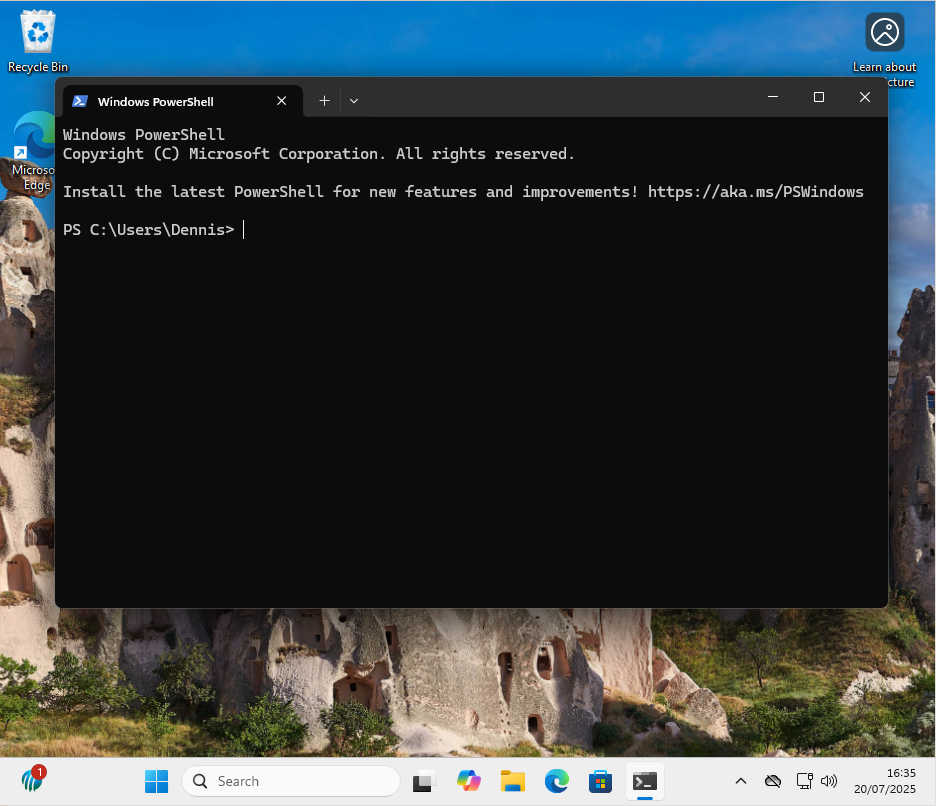
\includegraphics[width=0.99\linewidth]{Terminal_PS.png}%
}
\end{minipage}
Aan de linkerkant van het Terminal window zien we een knipperende cursor. Voor deze cursor vinden we een regel die begint met PS, om aan te geven dat we in PowerShell werken. Als er niets staat dan maken we gebruik van \texttt{cmd}. Na de PS zien we C:, dit is onze C-drive. Je kunt je nu afvragen waar de A en de B-drive gebleven zijn. Dat is geen vreemde vraag. Het Windows besturingssysteem bestaat al lang en in een grijs verleden waren er floppy disks en deze disks moest je plaatsen in een, meestal ingebouwde, floppy drive. De eerste twee drive letters waren gereserveerd voor deze floppy drives. De eerste harddisk in een systeem kreeg daardoor de letter C en dat is altijd zo gebleven. De C-drive is de disk waarvan het systeem is opgestart. Hierop staat Windows op en alles wat daarbij hoort.

Het laatste stuk bestaat uit \texttt{\textbackslash Users\textbackslash Username}. Dit is het pad waarin je staat. Username is bij jou vervangen door de naam waarmee je ingelogd bent. Als je ingelogd bent als Administrator dan is het pad: \texttt{\textbackslash WINDOWS\textbackslash system32}. In de laatste geval adviseren zou je eigenlijk moeten uitloggen en inloggen als gewone gebruiker. Als Administrator heb je te veel rechten en kan je te veel stuk maken.


\subsection{Werken met files en folders}
De data op een disk (harddisk of SSD) is verdeeld over mappen\index{mappen}, folders\index{folders} of directories\index{directories}. Deze namen worden door elkaar gebruikt, maar betekenen allemaal hetzelfde. Het zijn plekken waar bestanden\index{bestanden} of in het Engels files\index{files} in kunnen worden opgeslagen zodat de data op de disk overzichtelijk kan worden ingedeeld. De directory waarin je nu staat is je home-directory\index{home-directory}, de plek waar jij je bestanden in mag opslaan.

Om de organisatie van data te bevorderen heeft Microsoft al een aantal subdirectories voor je aangemaakt. Type op de prompt \texttt{dir}\index{dir}\index{commando!dir} en geef enter. Je krijgt nu een overzicht van bestanden en directories in jouw home-directory, zoals \texttt{Downloads}, \texttt{Documents}, \texttt{Music}, \texttt{Pictures}, \texttt{Videos} en nog wat meer. De hoop is dat gebruikers op deze manier hun data gestructureerd opslaan. Je hoeft je niet aan de structuur van Microsoft te houden. Als jij liever je data indeelt op basis van \texttt{Prive}, \texttt{School}, \texttt{Werk} kan dat natuurlijk ook. Alleen moet je dan nog wel zelf die directories maken.

Met het \texttt{mkdir}\index{mkdir}\index{commando!mkdir} commando kan je een directory aanmaken:
\begin{lstlisting}[style=DOS]
mkdir Prive
\end{lstlisting}

Met het \texttt{rmdir}\index{rmdir}\index{commando!rmdir} commando kan je een directory weggooien:
\begin{lstlisting}[style=DOS]
rmdir Prive
\end{lstlisting}
Directories die we met \texttt{rmdir} weggooien komen niet in de Recycle Bin terecht zoals dat wel gebeurt als je dat via \texttt{File Explorer} zou doen.

Je kan een directory alleen weggooien als deze leeg is. Alle default door Microsoft aangemaakte directories zijn niet leeg. Ze bevatten subdirectories of verborgen bestanden. Met de \texttt{-hidden} optie kan je met \texttt{dir} deze verbonden bestanden zichtbaar maken. Doen we een
\begin{lstlisting}[style=DOS]
dir Videos
\end{lstlisting}
Dan lijkt deze map leeg. Doen we echter:
\begin{lstlisting}[style=DOS]
dir -hidden Videos
\end{lstlisting}
Dan zie je dat er een bestand zichtbaar is geworden, namelijk een \texttt{desktop.ini} file.

We hebben gezien dat we met \texttt{rmdir} directories weg kunnen gooien. Met het \texttt{del}\index{del}\index{commando!del} commando kan je bestanden weggooien, ook deze komen niet in de Recycle Bin terecht en zijn direct van het systeem verdwenen.

Om met mappen en bestanden om te kunnen gaan in PowerShell is er nog een commando nodig dat je veel zult gebruiken en dat commando is \texttt{cd}\index{cd}\index{commando!cd}, wat een afkorting is van Change Directory. Daarmee kan je dus van directory wijzigen.

\begin{lstlisting}[style=DOS]
cd Documents
dir
\end{lstlisting}
De bovenstaande commando's zorgen ervoor dat je eerst jezelf verplaatst naar de Documents directory (LET OP: je prompt wijzigt mee) en met \texttt{dir} laat je zien welke files en folders er in deze directory staan. Je mag aan \texttt{cd} ook een volledig pad meegeven. Bijvoorbeeld
\begin{lstlisting}[style=DOS]
cd \Users
\end{lstlisting}
en met .. gaan we stapje dichter naar de basis van de harddisk, namelijk de root directory (\textbackslash).



\section{Directory structure}
De manier waarop bestanden en mappen zijn ingedeeld op een disk noemen we een directory-tree\index{directory-tree}. De tree begint bij de root. De root directory\texttt{root directory} is de directory die direct na de C: komt en wordt weergegeven door een enkele \textbackslash. We kunnen snel daar de root-directory gaan met:
\begin{lstlisting}[style=DOS]
cd \
\end{lstlisting}
We staan nu aan het begin van de directory boom van de C-schijf. Met \texttt{dir} kunnen we zien welke directories er de eerste takken van de boom vormen:

\begin{minipage}[t]{\linewidth}
\raggedright
\adjustbox{valign=t}{%
	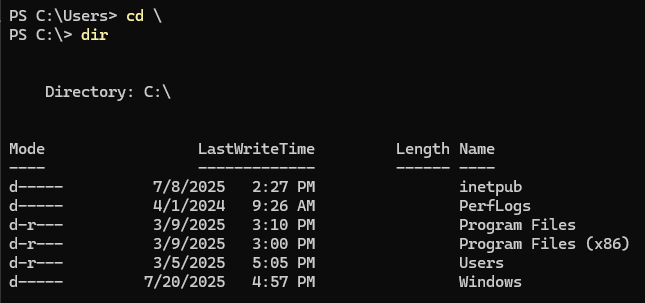
\includegraphics[width=0.99\linewidth]{Windows-rootdirs.png}%
}
\end{minipage}

\subsection{\textbackslash Windows}
De \texttt{Windows} directory bevat alles wat bij het besturingssysteem behoort. Wijzigingen aanbrengen in deze tak van de directory tree kan je Windows systeem mogelijk stuk maken. Maar het is wel goed om te weten wat je zoal in deze tak kan aantreffen.

Windows gebruikt extensies om aan te geven om wat voor soort bestanden het gaat. De extentie .docx geeft aan dat het om en Microsoft Word bestand gaat in XML-formaat. Zo zijn er vele extensies, we zullen er hier een aantal noemen die je op het systeem regelmatig tegen zult komen:
\begin{description}
\item[exe] Een executable, dat wil zeggen dat het een commando of een applicatie is die je kan opstarten als je de juiste rechten daarvoor hebt.
\item[log] Een log bestand. Bevat informatie over wat er op het systeem gebeurd is.
\item[dll] Een dynamic loadable library. Wordt gebruikt door applicaties of commando's.
\item[txt] Een text bestand zonder opmaak van de tekst.
\item[ini] Een configuratie bestand. Wijzigingen in dit bestand kunnen de manier waarop het systeem werkt veranderen. Met het \texttt{type} commando kan je de inhoud van een ini of een txt bestand laten zien op het scherm. Met \texttt{notepad} kan je ini en txt bestanden wijzigen.
\end{description}

De \texttt{Windows} directory bevat heel veel subdirectories, die gaan we niet allemaal behandelen, maar een paar willen we hier wel benoemen:
\begin{description}
\item[\textbackslash Windows\textbackslash System32] Bevat executables en libraries die cruciaal zijn voor de werking van het Windows systeem. Hoewel het lijkt of het 32-bits is, wordt de folder gebruikt voor 64-bits zaken.
\item[\textbackslash Windows\textbackslash SysWOW64] Een 64-bit operating system kan ook 32-bit applicaties draaien. Op een 64-bit Windows versie vind je de \texttt{SysWOW64} folder met daarin de 32-bits files en resources die nodig zijn voor het besturingssysteem. De \texttt{SysWOW64} folder is feitelijk de oude \texttt{System32} folder met daarin de 32-bits zaken.
\end{description}


\subsection{\textbackslash Program Files}
De \texttt{Program Files}\index{Program Files} directory is de plek waar applicaties die niet onderdeel zijn van het besturingssysteem worden ge\"installeerd. Windows 64-bits kan ook Windows 32-bits applicaties draaien. Om deze twee soorten bestanden uit elkaar te houden zijn er op een 64-bits systeem twee \texttt{Program Files} directories, een 32-bits Windows systeem kent er maar \'e\'en.

De applicaties die gebouwd zijn met het aantal bits dat behoort bij het OS worden ge\"installeerd in de \texttt{\textbackslash Program Files}, voor een 32-bits systeem zijn dat de 32-bits applicaties en voor een 64-bits systeem zijn dat de 64-bits applicaties.

De 32-bits applicaties op een 64-bits systeem worden ge\"installeerd in de \texttt{\textbackslash Program Files (x86)} directory. Een 32-bits systeem kent deze directory niet.


\subsection{\textbackslash Users}
De \texttt{\textbackslash Users} directory bevat de subdirectories voor alle gebruikers op een systeem. Elke gebruiker heeft zijn eigen directory met daarin zijn of haar documenten.



%%%%%%%%%%%%%%%%%%%%%
%%% Index and End %%%
%%%%%%%%%%%%%%%%%%%%%
\printindex
\end{document}

%%% Last line %%%
